

\chapter[Proof techniques I]{Proof techniques I --- Standard methods}
%\label{ch:proof1}

As a convenience, the table containing the definitions of elementary number theory is reproduced on the following page.

\begin{table}[hbt] 
\begin{center}
\begin{tabular}{l}
\rule{12pt}{0pt} Even \\
\framebox{\begin{minipage}{.8\textwidth}%
\rule[-6pt]{0pt}{20pt} $\forall n \in \Integers$, \\
\centerline{\rule[-6pt]{0pt}{20pt}$n$ is even \rule{6pt}{0pt} $\iff$ \rule{6pt}{0pt} $\exists  k \in \Integers, \; n = 2k$} \end{minipage} }\\
\rule{12pt}{0pt} Odd \\
\framebox{\begin{minipage}{.8\textwidth}%
\rule[-6pt]{0pt}{20pt} $\forall n \in \Integers$, \\
\centerline{\rule[-6pt]{0pt}{20pt}$n$ is odd \rule{6pt}{0pt} $\iff$ \rule{6pt}{0pt} $\exists
 k \in \Integers, \; n = 2k+1$} \end{minipage} }\\
\rule{12pt}{0pt} Divisibility\\
\framebox{\begin{minipage}{.8\textwidth}%
\rule[-6pt]{0pt}{20pt} $\forall n \in \Integers , \forall \quad d>0 \in \Integers$, \\
\centerline{\rule[-6pt]{0pt}{20pt}$d \divides n$  \rule{6pt}{0pt} $\iff$ \rule{6pt}{0pt} $\exists
 k \in \Integers, \; n = kd$} \end{minipage} } \\
\rule{12pt}{0pt} Floor\\
\framebox{\begin{minipage}{.8\textwidth}%
\rule[-6pt]{0pt}{20pt} $\forall x \in \Reals$, \\
\centerline{\rule[-6pt]{0pt}{20pt}$y = \lfloor x \rfloor$  \rule{6pt}{0pt} $\iff$ \rule{6pt}{0pt} 
$ y \in \Integers \, \; \land \, \; y \leq x < y+1$} \end{minipage} }\\
\rule{12pt}{0pt} Ceiling\\
\framebox{\begin{minipage}{.8\textwidth}%
\rule[-6pt]{0pt}{20pt} $\forall x \in \Reals$, \\
\centerline{\rule[-6pt]{0pt}{20pt}$y = \lceil x \rceil$  \rule{6pt}{0pt} $\iff$ \rule{6pt}{0pt} 
$ y \in \Integers \, \; \land \, \; y-1 < x \leq y$} \end{minipage} }\\
\rule{12pt}{0pt} Quotient-remainder theorem, Div and Mod\\
\framebox{\begin{minipage}{.8\textwidth}%
\rule[-6pt]{0pt}{20pt}$\forall n, d>0 \in \Integers$,\\
\centerline{\rule[-6pt]{0pt}{20pt}$\exists \mbox{!} q,r \in \Integers, \; n = qd + r \, \; \land \, \; 0 \leq r < d $} 
\rule[-6pt]{0pt}{20pt}\centerline{$n \; \mbox{div} \; d = q$} \newline
\rule[-6pt]{0pt}{20pt}\centerline{$n \; \mbox{mod} \; d = r$} 
\end{minipage} }\\
\rule{12pt}{0pt} Prime\\
\framebox{\begin{minipage}{.8\textwidth}%
\rule[-6pt]{0pt}{20pt}$\forall \, p \, \in \Integers$\\
\rule[-6pt]{0pt}{20pt}\centerline{$p$ is prime \rule{6pt}{0pt}%
$\iff$ \rule{60pt}{0pt} }
\rule[-6pt]{0pt}{12pt}\centerline{\rule{30pt}{0pt} $(p>1) \quad \land \quad (\forall x,y \in \Integers^+, \; p=xy \; \implies \; x=1 \, \lor \,  y=1)$} 
\end{minipage} }\\
\end{tabular}
\end{center}
\caption{The definitions of elementary number theory restated.}
\label{tab:defs}
\end{table}

\clearpage 

\section{Direct proofs of universal statements}
%\label{sec:direct}






\noindent{\large \bf Exercises --- \thesection\ }

\begin{enumerate}
\item Every prime number greater than 3 is of one of the two forms
$6k+1$ or $6k+5$.  What statement(s) could be used as hypotheses in
proving this theorem?

\hint{

\vfill

Fill in the blanks:
\begin{itemize}
\item $p$ is a \underline{\rule{1.5in}{0in}} number, and
\item $p$ is greater than \underline{\rule{1in}{0in}}.
\end{itemize}

\vfill

}

\item Prove that 129 is odd.

\hint{

\vfill

\rule{12pt}{0pt} All you have to do to show that some number is odd, is produce the integer $k$ that the definition
of ``odd'' says has to exist.  Hint: the same number could be used to prove that $128$ is even.

\vfill

}

\item Prove that the sum of two rational numbers is a rational number.

\hint{

\vfill

\rule{12pt}{0pt} You want to argue about the sum of two generic rational numbers. Maybe call them $a/b$ and $c/d$. The definition of ``rational number'' then tells you that $a$, $b$, $c$ and $d$ are integers and that neither $b$ nor $d$ are zero. You add these generic rational numbers in the usual way -- put them over a common denominator and then add the numerators. One possible common denominator is $bd$, so we can express the sum as $(ad+bc)/(bd)$.  You can finish off the argument from here: you need to show that this expression for the sum satisfies the definition of a rational number (quotient of integers w/ non-zero denominator). Also, write it all up a bit more formally\ldots

\vfill

}

\hintspagebreak

\item Prove that the sum of an odd number and an even number is odd.


\hint{

\vfill

\begin{proof}
Suppose that $x$ is an odd number and $y$ is an even number.  Since $x$ is odd there is an 
integer $k$ such that $x=2k+1$.  Furthermore, since $y$ is even, there is an integer $m$ such that
$y=2m$.  By substitution, we can express the sum $x+y$ as $x+y = (2k+1) + (2m) = 2(k+m) + 1$.
Since $k+m$ is an integer (the sum of integers is an integer) it follows that $x+y$ is odd.
\end{proof}

\vfill

}

\item Prove that if the sum of two integers is even, then so is their
difference.

\hint{

\vfill

Hint: If we write $x+y$ for the sum of two integers that is even (so $x+y = 2k$ for some integer $k$), then we could subtract \underline{\rule{1in}{0in}} from it in order to obtain $x-y$. Once you fill in that blank properly the flow of the argument should become apparent to you.

\vfill

}

\item Prove that for every real number $x$, $\frac{2}{3} < x < \frac{3}{4} \; \implies \; \lfloor 12x \rfloor = 8$.

\hint{

\vfill

Begin your proof like so:

``Suppose that $x$ is a real number such that $\frac{2}{3} < x < \frac{3}{4}$.''

You need to multiply all three parts of the inequality by something in order to ``clear'' the fractions.
What should that be?


The definition for the floor of $12x$ will be satisfied if $8 \leq 12x < 9$ but unfortunately the work done 
previously will have deduced that $8 < 12x < 9$ is true.  Don't just gloss over this discrepancy.  Explain why
one of these inequlities is implied by the other.

\vfill

}

\hintspagebreak

\item Prove that if $x$ is an odd integer, then $x^2$ is of the form
$4k+1$ for some integer $k$.

\hint{

\vfill

\rule{12pt}{0pt} You may be tempted to write ``Since x is odd, it can be expressed as $x = 2k+1$ where $k$ is an integer.'' This is slightly wrong since the variable $k$ is already being used in the statement of the theorem. But, except for replacing $k$ with some other variable (maybe $m$ or $j$?) that {\em is} a good way to get started. From there it's really just algebra until, eventually, you'll find out what $k$ really is.

\vfill

}

\item Prove that for all integers $a$ and $b$, if $a$ is odd and $6 \divides (a+b)$, then $b$ is odd.

\hint{

\vfill

\rule{12pt}{0pt} The premise that $6 \divides (a+b)$ is a bit of a red herring (a clue that is designed to mislead).  The premise that you really need is that $a+b$ is even.  Can you deduce that from what's given?

\vfill

}

\item Prove that $\forall x\in\Reals \, x\not\in\Integers \, \implies \, \lfloor x\rfloor+\lfloor-x\rfloor=-1$.

\hint{

\vfill

\begin{proof}
Suppose that $x$ is a real number and $x\not\in\Integers$.  Let $a = \lfloor x \rfloor$.  By the definition
of the floor function we have $a \in\Integers$ and $ a \leq x < a+1$.   Since $x \not\in\Integers$ we
know that $x \neq a$ so we may strengthen the inequality to $a < x < a+1$.  Multiplying this inequality
by $-1$ we obtain $-a > -x > -a - 1$.  This inequlity may be weakened to $-a > -x \geq -a - 1$.  Finally, note that (since $-a-1 \in\Integers$ and $-a = (-a-1)+1$ we
have shown that $\lfloor -x \rfloor \, = \, -a-1$.  Thus, by substitution we have $\lfloor x \rfloor+\lfloor -x \rfloor \; = \; a + (-a-1) \; = \; -1$ as desired.
\end{proof}

\vfill

}

\hintspagebreak

\item Define the \index{evenness}\emph{evenness} of an integer $n$ by:

\[ \mbox{evenness} (n) = k \; \iff \;  
 2^k \divides n \, \land \, 2^{k+1} \nmid n \]

State and prove a theorem concerning the evenness of products.

\hint{Well, the statement is that the evenness of a product is the sum of the evennesses of the factors\ldots}


\item Suppose that $a$, $b$ and $c$ are integers such that $a \divides b$
and $b \divides c$.  Prove that $a \divides c$.

\hint{
This one is pretty straightforward. Be sure to not reuse any variables. Particularly, the fact that $a \divides b$ tells us (because of the definition of divisibility) that there is an integer $k$ such that $b = ak$.  It is not okay to also use $k$ when converting the statement ``$b \divides c$.''
}

\textbookpagebreak

\item Suppose that $a$, $b$, $c$ and $d$ are integers with $a \neq c$.
Further, suppose that $x$ is a real number satisfying the equation

\[ \frac{ax+b}{cx+d} = 1. \]


\noindent Show that $x$ is rational.  Where is the hypothesis $a \neq c$
used?

\hint{Cross multiply and solve for $x$.  If you need to divide by an expression, it had 
better be non-zero!}

\item Show that if two positive integers $a$ and $b$ satisfy $a \divides b$ \emph{and}
$b \divides a$ then they are equal.

\hint{From the definition of divisibility, you get two integers $j$ and $k$, such that 
$a = jb$ and $b = ka$. Substitute one of those into the other and ask yourself what 
the resulting equation says about $j$ and $k$.  Can they be any old integers?  Or, are 
there restrictions on their values?
}

\end{enumerate}


\newpage
\section{More direct proofs}
%\label{sec:more}


\noindent{\large \bf Exercises --- \thesection\ }

\begin{enumerate}
\item Suppose you have a savings account which bears interest 
compounded monthly.  The July statement shows a balance of 
\$ 2104.87 and the September statement shows a balance \$ 2125.97.
What would be the balance on the (missing) August statement?

\hint{A savings account where we are not depositing or withdrawing funds has a balance that is growing geometrically.}

\item \label{quad} Recall that a quadratic equation $ax^2+bx+c=0$ has two real solutions
if and only if the discriminant $b^2-4ac$ is positive.  Prove that if 
$a$ and $c$ have different signs then the quadratic equation has two 
real solutions.

\hint{You don't need all the hypotheses. If $a$ and $c$ have different signs, then $ac$ is a negative quantity}

\item Prove that if $x^3-x^2$ is negative then $3x+4 < 7$.

\hint{This follows very easily by the method of working backwards from the conclusion. Remember that when multiplying or dividing both sides of an inequality by some number, the direction of the inequality may reverse (unless we know the number involved is positive).  Also, remember that we can't divide by zero, so if we are (just for example, don't know why I'm mentioning it really\ldots) dividing both sides of an inequality by $x^2$ then we must treat the case where $x=0$ separately.}

\item Prove that for all integers $a,b,$ and $c$, if $a|b$ and $a|(b+c)$, then
$a|c$.

\item Show that if $x$ is a positive real number, then $x+\frac{1}{x} \geq 2$. 

\hint{If you work backwards from the conclusion on this one, you should eventually come to the inequality $(x-1)^2 \geq 0$.  Notice that this inequality is always true -- all squares are non-negative. When you go to write-up your proof (writing things in the forward direction), you'll want to acknowledge this truth. Start with something like ``Regardless of the value of $x$, the quantity $(x-1)^2$ is greater than or equal to zero as it is a perfect square.''}

\item Prove that for all real numbers $a,b,$ and $c$, if $ac<0$, then the quadratic
equation $ax^{2}+bx+c=0$ has two real solutions.\\
\textbf{Hint:} The quadratic equation $ax^{2}+bx+c=0$ has two
real solutions if and only if $b^{2}-4ac>0$ and $a\neq0$.

\hint{This is very similar to problem \ref{quad}.}

\item Show that $\binom{n}{k} \cdot \binom{k}{r} \; = \; \binom{n}{r} \cdot \binom{n-r}{k-r}$ (for all integers $r$, $k$ and $n$ with $r \leq k \leq n$). 

\hint{Use the definition of the binomial coefficients as fractions involving factorials:

E.g. $\displaystyle\binom{n}{k} \; = \; \frac{n!}{k! (n-k)!}$

Write down the definitions, both of the left hand side and the right hand side and consider how you can
convert one into the other.}

\item In proving the \index{product rule} \emph{product rule} in Calculus using the definition of the derivative, we might start our proof with:

\[
\frac{\mbox{d}}{\mbox{d}x} \left( f(x) \cdot g(x) \right)
\]

\[ = \lim_{h \longrightarrow 0} \frac{f(x+h) \cdot g(x+h) - f(x) \cdot g(x)}{h} \]

\noindent The last two lines of our proof should be:
\[
= \lim_{h \longrightarrow 0} \frac{f(x+h) - f(x)}{h} \cdot g(x) \; + \; f(x) \cdot \lim_{h \longrightarrow 0} \frac{g(x+h) - g(x)}{h}
\]

\[
= \frac{\mbox{d}}{\mbox{d}x}\left( f(x) \right) \cdot g(x) \; + \; f(x) \cdot \frac{\mbox{d}}{\mbox{d}x}\left( g(x) \right) 
\]

Fill in the rest of the proof.

\hint{The critical step is to subtract and add the same thing: $f(x)g(x+h)$ in the numerator of the fraction
in the limit which gives the definition of $\frac{\mbox{d}}{\mbox{d}x} \left( f(x) \cdot g(x) \right)$.  Also, you'll need to recall the laws of limits (like ``the limit of a product is the product of the limits -- provided both exist'') }

\end{enumerate}

\newpage

\section[Contradiction and contraposition]{Indirect proofs: contradiction and contraposition}
%\label{sec:contra}

\noindent{\large \bf Exercises --- \thesection\ }

\begin{enumerate}
\item Prove that if the cube of an integer is odd, then that integer is odd.

\hint{The best hint for this problem is simply to write down the contrapositive statement. It is trivial to prove!}

\item Prove that whenever a prime $p$ does not divide the square of an integer, 
it also doesn't divide the original integer. 
($p \nmid x^2 \; \implies \; p \nmid x$)

\hint{The contrapositive is $(p \divides x) \; \implies \; (p \divides x^2)$.}

\item Prove (by contradiction) that there is no largest integer.

\hint{Well, if there was a largest integer -- let's call it $L$ (for largest) -- then isn't $L+1$ an integer, and isn't it bigger?  That's the main idea.  A more formal proof might look like this:

\begin{proof} 
Suppose (by way of contradiction) that there is a largest integer $L$.   Then $L \in \Integers$ and $\forall z \in \Integers, L \geq z$.
Consider the quantity $L+1$.  Clearly $L+1$ is an integer (because it is the sum of two integers) and also
$L+1 > L$.   This is a contradiction so the original supposition is false.   Hence there is no largest integer.
\end{proof}
}

\item Prove (by contradiction) that there is no smallest positive real number.

\hint{Assume there was a smallest positive real number -- might as well call it $s$ (for smallest) -- what can we do to produce an even smaller number? (But be careful that it needs to remain positive -- for instance $s-1$ won't work.)}

\item Prove (by contradiction) that the sum of a rational and an irrational 
number is irrational.

\hint{Suppose that x is rational and y is irrational and their sum (let's call it z) is also rational. Do some algebra to solve for y, and you will see that y (which is, by presumption, irrational) is also the difference of two rational numbers (and hence, rational -- a contradiction.)

}

\item Prove (by contraposition) that for all integers $x$ and $y$, if $x+y$ is odd, then $x\neq y$.

\hint{Well, the problem says to do this by contraposition, so let's write down the contrapositive:

\[ \forall x, y \in \Integers, \; x=y \, \implies \, x+y \; \mbox{is even}. \]

But proving that is obvious!
}

\item Prove (by contraposition) that for all real numbers $a$ and $b$, if $ab$ is irrational, then $a$
is irrational or $b$ is irrational.

\hint{The contrapositive would be:

\[ \forall a,b \in \Reals, \; (a \in \Rationals \land b \in \Rationals) \, \implies ab \in \Rationals. \]

Wow! Haven't we proved that before?}

\item A \index{Pythagorean triple}\emph{Pythagorean triple} is a set of three
natural numbers, $a$, $b$ and $c$, such that $a^2 + b^2 = c^2$.  Prove that, in a
Pythagorean triple, at least one of $a$ and $b$ is even.  Use either a proof by
contradiction or a proof by contraposition.

\hint{If both $a$ and $b$ are odd then their squares will be 1 mod 4 -- so the sum of their squares
will be 2 mod 4.  But $c^2$ can only be 0 or 1 mod 4, which gives us a contradiction.}

\item Suppose you have 2 pairs of positive real numbers whose products are 1.  That is, you have $(a,b)$ and $(c,d)$ in $\Reals^2$ satisfying $ab=cd=1$.  Prove that
$a < c$ implies that $b > d$.

 \hint{
 \begin{proof}
 Suppose by way of contradiction that $a,b,c,d \in \Reals$ satisfy $ab=cd=1$ and that $a<c$ and $b \leq d$.
 By multiplying the inequalities we get that $ab < cd$ which contradicts the assumption that both products
 are equal to 1 (and so must be equal to one another).
 \end{proof} 
  } 
\end{enumerate}


\newpage

\section{Disproofs}
%\label{sec:disproofs}


\noindent{\large \bf Exercises --- \thesection\ }

\begin{enumerate}
\item Find a polynomial that assumes only prime values for
a reasonably large range of inputs.

\hint{It sort of depends on what is meant by ``a reasonably large range of inputs.''  For example the polynomial $p(x) = 2x+1$ gives primes three times in a row (at $x=1,2$ and $3$).  See if you can do better than that.
}

\wbvfill

\item Find a counterexample to \ifthenelse{\boolean{InTextBook}}{Conjecture~\ref{conj:prim}}{the conjecture that $\forall a,b,c \in \Integers, a \divides bc \; \implies \; a \divides b \, \lor \, a \divides c$} using only powers of 2.

\hint{The intent of the problem is that you find three numbers, $a$, $b$ and $c$, that are all powers 
of $2$ and such that $a$ divides the product $bc$, but neither of the factors separately. For instance, 
if you pick $a=16$, then you would need to choose $b$ and $c$ so that $16$ doesn't divide evenly 
into them (they would need to be less than $16$\ldots) but so that their product {\em is} divisible by $16$.
}

\wbvfill

\workbookpagebreak

\item The alternating sum of factorials provides an interesting
example of a sequence of integers.
\begin{center}
\[ 1! = 1 \]
\[ 2! - 1! = 1\]
\[ 3! - 2! + 1! = 5 \]
\[ 4! - 3! + 2! - 1! = 19 \]
et cetera
\end{center}

\noindent Are they all prime?  (After the first two 1's.)

\hint{

Here's some Sage code that would test this conjecture:

{\tt 
n=1\newline
for i in [2..8]:\newline
    n = factorial(i) - n\newline
    show(factor(n))\newline
}

Of course it turns out that going out to $8$ isn't quite far enough\ldots

}

\wbvfill

\item It has been conjectured that whenever $p$ is prime, $2^p - 1$ is
also prime.  Find a minimal counterexample.

\hint{I would definitely seek help at your friendly neighborhood CAS.  In Sage 
you can loop over the first several prime numbers using the following syntax.

{\tt for p in [2,3,5,7,11,13]:}

\noindent If you want to automate that somewhat, there is a Sage function that returns a list
of all the primes in some range.  So the following does the same thing.

{\tt for p in primes(2,13):}
}

\wbvfill

\workbookpagebreak

\item True or false:  The sum of any two irrational numbers is irrational.
Prove your answer.

\hint{This statement and the next are negations of one another.  Your answers should reflect that.}

\wbvfill

\item True of false:  There are two irrational numbers whose sum is rational.
Prove your answer.

\hint{If a number is irrational, isn't its negative also irrational?  That's actually a pretty huge hint.}

\wbvfill

\item True or false: The product of any two irrational numbers is irrational.
Prove your answer.

\hint{This one and the next are negations too. Aren't they?}

\wbvfill

\item True or false: There are two irrational numbers whose product is rational.
Prove your answer.

\hint{The two numbers {\em could} be equal couldn't they?}

\wbvfill

\item True or false:  Whenever an integer $n$ is a divisor of the square of an integer, $m^2$, it follows that $n$ is a divisor of $m$ as well.
(In symbols, $\forall n \in \Integers, \forall m \in \Integers, n \mid m^2 \; \implies \; n \mid m$.)
Prove your answer.

\hint{Hint: List all of the divisors of $36 = (2\cdot 3)^2$.  See if any of them are bigger than $6$.}

\wbvfill

\workbookpagebreak

\item In an exercise in Section~\ref{sec:more} we proved that the quadratic 
equation $ax^2 + bx + c = 0$ has two solutions if $ac < 0$.  Find a counterexample which shows that this implication cannot be replaced with a biconditional.  

\hint{We'd want $ac$ to be positive (so $a$ and $c$ have the same sign) but nevertheless have $b^2-4ac > 0$.  It seems that if we make $b$ sufficiently large that could happen.}

\wbvfill

\end{enumerate}


\newpage

\section[By cases and By exhaustion]{Even more direct proofs: By cases and By exhaustion}
%\label{sec:cases}


\noindent{\large \bf Exercises --- \thesection\ }

\begin{enumerate}
\item Prove that if $n$ is an odd number then $n^4 \pmod{16} = 1$.

\hint{

While one could perform fairly complicated arithmetic, expanding expression like
$(16k+13)^4$ and then regrouping to put it in the form $16q+1$ (and one would need 
to do that work for each of the odd remainders modulo $16$),  that would be missing out
on the true power of modular notation.  In a ``$\pmod{16}$'' calculation one can simply ignore
summands like $16k$ because they are $0 \pmod{16}$.  Thus, for example,

  \[ (16k+7)^4 \pmod{16} \; = \; 7^4 \pmod{16} \; = \; 2401 \pmod{16}  \; = \; 1. \]
  
So, essentially one just needs to compute the $4$th powers of $1, 3, 5, 7, 9, 11, 13$  and $15$, and
then reduce them modulo 16.  An even greater economy is possible if one notes that (modulo 16) many
of those cases are negatives of one another -- so their $4$th powers are equal.
}

\wbvfill
     
\item Prove that every prime number other than 2 and 3 has the form
$6q+1$ or $6q+5$ for some integer $q$.  (Hint: this problem involves
thinking about cases as well as contrapositives.)

\hint{It is probably obvious that the "cases" will be the possible remainders mod 6. Numbers of the form 6q+0 will be multiples of 6, so clearly not prime. The other forms that need to be eliminated are 6q+2, 6q+3, and 6q+4.
}

\wbvfill

\workbookpagebreak

\item Show that the sum of any three consecutive integers is divisible
by 3.

\hint{Write the sum as $n + (n+1) + (n+2)$.}

\wbvfill

\item There is a graph known as $K_4$ that has $4$ nodes and there is an edge between every pair of nodes.
The pebbling number of $K_4$ has to be at least $4$ since it would be possible to put one pebble on each of
$3$ nodes and not be able to reach the remaining node using pebbling moves.  Show that the pebbling number of $K_4$ is actually $4$.

\hint{If there are two pebbles on any node we will be able to reach all the other nodes using pebbling moves
(since every pair of nodes is connected).}

\wbvfill

\workbookpagebreak

\item Find the pebbling number of a graph whose nodes are the corners and 
whose edges are the, uhmm, edges of a cube.

\hint{It should be clear that the pebbling number is at least $8$ -- $7$ pebbles could be distributed, 
one to a node, and the $8$th node would be unreachable.  It will be easier to play around with this if
you figure out how to draw the cube graph ``flattened-out'' in the plane.}

\wbvfill

\item A \index{vampire number}\emph{vampire number} is a $2n$ digit number $v$ that factors as $v=xy$
where $x$ and $y$ are $n$ digit numbers and the digits of $v$ are the 
union of the digits in $x$ and $y$ in some order.  The numbers $x$ and $y$
are known as the ``fangs'' of $v$.  To eliminate trivial
cases, pairs of trailing zeros are disallowed.  

Show that there are no 2-digit vampire numbers.

Show that there are seven 4-digit vampire numbers.

\hint{The 2-digit challenge is do-able by hand (just barely).  The $4$ digit question certainly requires 
some computer assistance!}

\wbvfill

\workbookpagebreak

\item Lagrange's theorem on representation of integers as sums of squares
says that every positive integer can be expressed as the sum of at most 
$4$ squares.  For example, $79 = 7^2 + 5^2 + 2^2 + 1^2$.  Show (exhaustively) 
that $15$ can not be represented using fewer than $4$ squares.

\hint{Note that $15 = 3^2 + 2^2 + 1^2 + 1^2$.  Also, if $15$ were expressible as a sum of fewer than $4$ squares, the squares involved would be $1$, $4$ and $9$.  It's really not that hard to try all the possibilities.}

\wbvfill

\item Show that there are exactly $15$ numbers $x$ in the range $1 \leq x \leq 100$ that can't be represented using fewer than $4$ squares.



\hint{The following Sage code generates all the numbers up to $100$ that {\em can} be written
as the sum of at most $3$ squares.

{\tt
var('x y z') \newline
a=[s$\caret$2 for s in [1..10]]  \newline
b=[s$\caret$2 for s in [0..10]]  \newline
s = []  \newline
for x in a:  \newline
\tab for y in b:  \newline
\tab \tab for z in b:  \newline
\tab \tab \tab s = union(s,[x+y+z])  \newline
s = Set(s)  \newline
H=Set([1..100]) \newline
show(H.intersection(s))  \newline
}
}

\wbvfill

\workbookpagebreak

\item The \index{trichotomy property}\emph{trichotomy property} of the real 
numbers simply states that every real number is either positive or negative 
or zero.  Trichotomy can be used to prove many statements by looking at the
three cases that it guarantees.  Develop a proof (by cases) that the square of
any real number is non-negative.

\hint{By trichotomy, x is either zero, negative, or positive. If x is zero, its square is zero. If x is negative, its square is positive. If x is positive, its square is also positive.}

\wbvfill

\hintspagebreak

\item Consider the game called ``binary determinant tic-tac-toe''\ifthenelse{\boolean{InTextBook}}{\footnote{ %
This question was problem A4 in the 63rd annual %
\index{William Lowell Putnam Mathematics Competition} %
William Lowell Putnam Mathematics Competition (2002).  %
There are three collections of questions %
and answers  from previous Putnam exams available from the MAA % 
\cite{putnam1,putnam2,putnam3}% 
}}{} 
which is played by two players who alternately fill in the entries of a 
$3 \times 3$ array.  Player One goes first, placing 1's in the array and 
player Zero goes second, placing 0's.  Player One's goal is that the 
final array have determinant 1, and player Zero's goal is that the 
determinant be 0.  The determinant calculations are carried out mod 2.

Show that player Zero can always win a game of binary determinant tic-tac-toe
by the method of exhaustion.

\hint{If you know something about determinants it would help here.  The determinant will be
0 if there are two identical rows (or columns) in the finished array.  Also, if there is a row or column
that is all zeros, player Zero wins too.  Also, cyclically permuting either rows or columns has no effect
on the determinant of a binary array.  This means we lose no generality in assuming player One's
first move goes (say) in the upper-left corner.}

\wbvfill

\workbookpagebreak

\rule{0pt}{0pt}

\workbookpagebreak

\end{enumerate}


\newpage

\section[Existential statements]{Proofs and disproofs of existential statements}
%\label{sec:exist}


\noindent{\large \bf Exercises --- \thesection\ } 

\begin{enumerate}
\item Show that there is a perfect square that is the sum of two
perfect squares.

\hint{Can you say "Pythagorean triple"? I thought you could.}

\wbvfill

\item Show that there is a perfect cube that is the sum of three
perfect cubes.

\hint{Hint: $6^3$ can be expressed as such a sum.}

\wbvfill

\workbookpagebreak

\item Show that the \index{well-ordering principle}WOP doesn't hold in the integers.  (This is an
existence proof, you show that there is a subset of $\Integers$
that doesn't have a smallest element.)

\hint{How about even integers? Is there a smallest one?  That's my example!  You come up with a 
different one!}

\wbvfill

\item Show that the WOP doesn't hold in $\Rationals^+$.

\hint{Consider the set $\{ 1, 1/2, 1/4, 1/8, \ldots \}$.  Does it have a smallest element?}

\wbvfill

\workbookpagebreak

\item In the proof of Theorem~\ref{gcd!exists} we weaseled out of
showing that $d \divides b$.  Fill in that part of the proof.

\hint{Yeah, I'm going to keep weaseling\ldots}

\wbvfill

\item Give a proof of the unique existence of $q$ and $r$ in the
division algorithm. 

\hint{Unique existence proofs consist of two parts. First, just show existence. Then, show that if there were two of the things under consideration that they must in fact be equal.}

\wbvfill

\workbookpagebreak

\item A \index{digraph}\emph{digraph} is a drawing containing a collection of points
that are connected by arrows.  The game known as \emph{scissors-paper-rock}
can be represented by a digraph that is \emph{balanced} (each point has the
same number of arrows going out as going in).  Show that there is a 
balanced digraph having 5 points.

\begin{center}
\begin{picture}(0,0)%
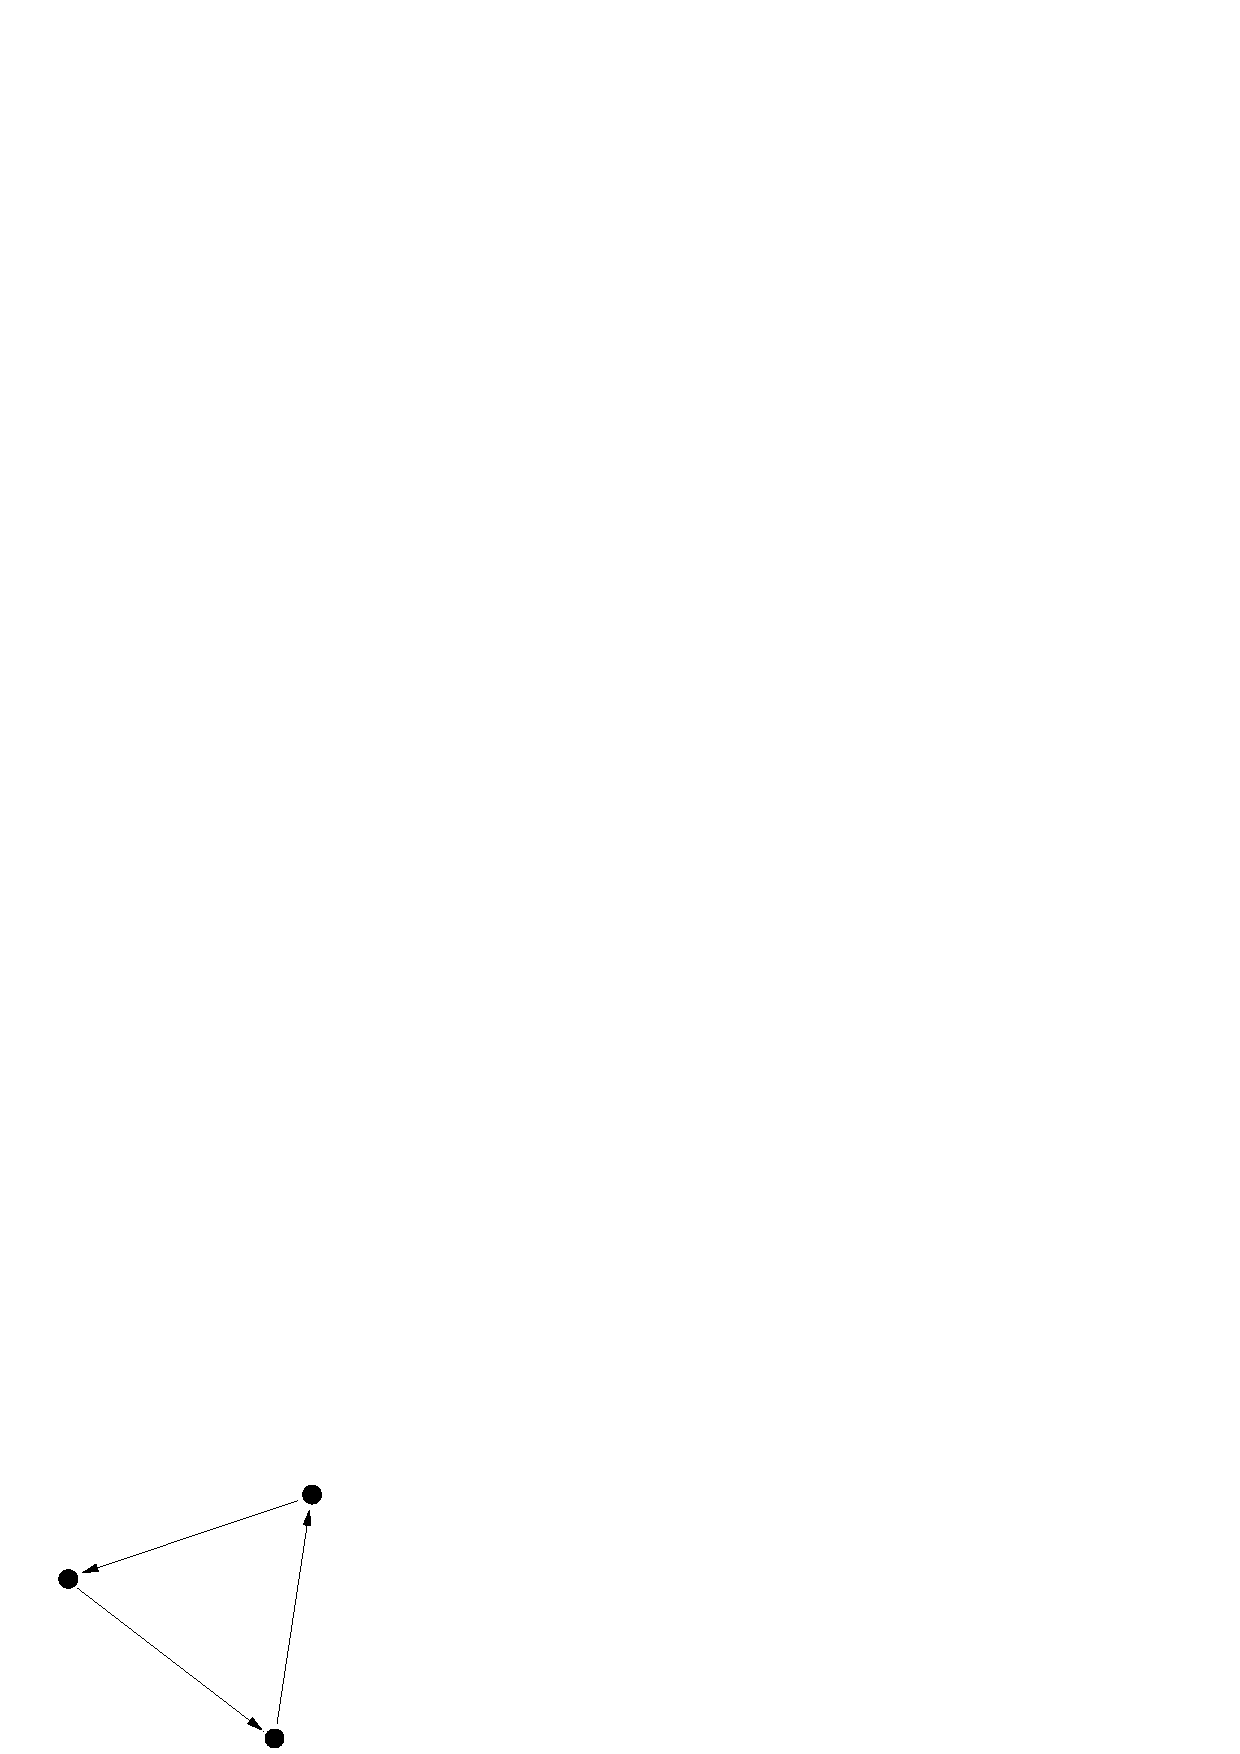
\includegraphics{figures/sci-pap-roc.pdf}%
\end{picture}%
\setlength{\unitlength}{3947sp}%
%
\begingroup\makeatletter\ifx\SetFigFont\undefined%
\gdef\SetFigFont#1#2#3#4#5{%
  \reset@font\fontsize{#1}{#2pt}%
  \fontfamily{#3}\fontseries{#4}\fontshape{#5}%
  \selectfont}%
\fi\endgroup%
\begin{picture}(3345,2223)(3054,-2286)
\put(5469,-1199){\makebox(0,0)[lb]{\smash{{\SetFigFont{12}{14.4}{\familydefault}{\mddefault}{\updefault}{\color[rgb]{0,0,0}smashes}%
}}}}
\put(5723,-213){\makebox(0,0)[lb]{\smash{{\SetFigFont{12}{14.4}{\familydefault}{\mddefault}{\updefault}{\color[rgb]{0,0,0}scissors}%
}}}}
\put(5381,-2271){\makebox(0,0)[lb]{\smash{{\SetFigFont{12}{14.4}{\familydefault}{\mddefault}{\updefault}{\color[rgb]{0,0,0}rock}%
}}}}
\put(3956,-1652){\makebox(0,0)[lb]{\smash{{\SetFigFont{12}{14.4}{\familydefault}{\mddefault}{\updefault}{\color[rgb]{0,0,0}covers}%
}}}}
\put(4423,-463){\makebox(0,0)[lb]{\smash{{\SetFigFont{12}{14.4}{\familydefault}{\mddefault}{\updefault}{\color[rgb]{0,0,0}cuts}%
}}}}
\put(3069,-837){\makebox(0,0)[lb]{\smash{{\SetFigFont{12}{14.4}{\familydefault}{\mddefault}{\updefault}{\color[rgb]{0,0,0}paper}%
}}}}
\end{picture}%

\end{center}
  
\hint{If at first you don't succeed\ldots \newline
try googling ``scissor paper rock lizard spock.''}

\wbvfill

\workbookpagebreak

\end{enumerate}


%\newpage
%\renewcommand{\bibname}{References for chapter 3}
%\bibliographystyle{plain}
%\bibliography{main}

%% Emacs customization
%% 
%% Local Variables: ***
%% TeX-master: "GIAM-hw.tex" ***
%% comment-column:0 ***
%% comment-start: "%% "  ***
%% comment-end:"***" ***
%% End: ***
 
